%Chapter describing the mimetic process
\chapter{The Inspiration: Mimicry}
\label{chapter:mimicry}
\begin{quote}
\textsl{``It is not the strongest of the species that survives, nor the most intelligent that survives. It is the one that is the most adaptable to change." - Charles Darwin}
\end{quote}

\section{History}
Henry W. Bates first published in 1862 his findings about the similarities and dissimilarities between Heliconiinae and Ithomiinae butterflies, after 10 years of research in the Brazilian rain forest. For the next hundred years, it simulated heated discussion among all groups of people, scientists, philosophers, theologians, teachers and amateur naturalists. Bates collected ninety-four pieces of butterfly. He grouped them according to their similar appearance. He found butterflies having similar appearance, exhibiting morphological features which point to completely different species even families. Out of the ninety four species, sixty seven are now classified as Ithomiinae, while twenty seven of them are Heliconiinae.

\section{Batesian Mimicry}
Even though Heliconiids are conspicuously colored, they are extremely abundant. They are also slow in mobility. Still predators in the surrounding area, mostly insectivorous birds do not prey on them, because of their inedible and unpalatable nature. Also because of this phenomenon other edible and palatable species such as ithomiinae and pieridae, pretend to be heliconiids and thus enjoy protection.

Repulsive animals, such as heliconiids are very conspicuously colored. Having this noticeable property, they are easily recalled by predators. Their wing pattern works as a warning to predators. Once a predator has the knowledge of their inedible and unpalatable property, they would probably never attempt to try it again. As this is true, if any organism within close family and species, but being edible and having a deceptive resemblance to those conspicuously colored species will be avoided by the predators. Wickler \cite{wickler1986} expresses,
\begin{quote}
\textsl{``Such unpalatable appearing and yet edible animals thus possess a false warning pattern, they 'act a part'. An actor is a mime, and so the representation of a false warning pattern was called \textit{mimicry}. Since Bates was the first to point out this phenomenon, it has received the name \textit{Batesian Mimicry} in his honor."}
\end{quote}
In general, the animal which is avoided by predator for unpalatable behavior is called the \textbf{model} and the imitating animal is called the \textbf{mimic}.

\begin{figure}[H]
	\centering
	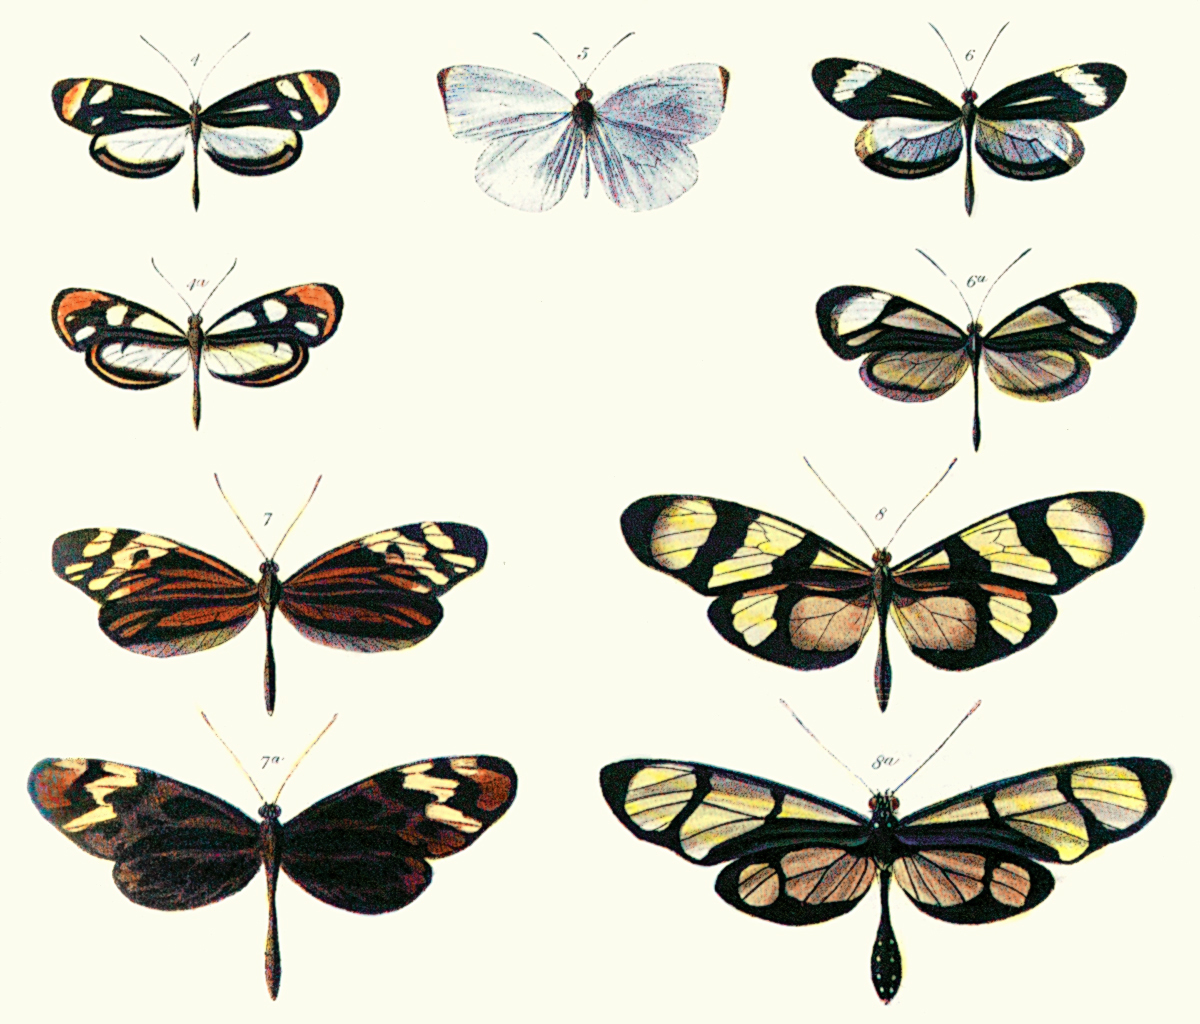
\includegraphics[scale=1]{images/Batesplate_ArM}
	\caption[Plate from Bates (1862) illustrating Batesian mimicry]{Plate from Bates (1862) illustrating Batesian mimicry between Dismorphia species (top row, third row) and various Ithomiini (Nymphalidae) (second row, bottom row). \cite{bates1862}}
	\label{fig:batesian-butterfly}
\end{figure}

\subsection{Definitions of Mimicry}
The following account on the definition of Mimicry is mostly extracted from Wickler's \textit{Mimicry in plants and animals} \cite{wickler1986}. 

According to Wickler the definition of mimicry provided by Bates \cite{bates1862} is quite restricted and is similar to the following

\begin{quote}
\textsl{``resemblance in external appearance, shapes and colors between members of widely distinct families."}
\end{quote}

The following more sophisticated definition was provided at the international Zoological Congress in Washington, 1963,

\begin{quote}
\textsl{``Mimicry is the close resemblance of one organism to another which, because it is unpalatable and conspicuous, is recognized and avoided by some predators at some times."}
\end{quote}

The best known definition of mimicry quoted to the present day, are those given by Wallace and listed in Poulton's \textit{The color of animals, their meaning and use} \cite{poulton1890colours}. The clauses are presented in the following:

\begin{itemize}
	\item \textsl{``that the imitative species occur in the same area and occupy the same station as the imitated".} This increases the probability that a predator will affect both parties concerned. Nevertheless, the model could live in Africa and the mimic in Europe, or vice versa, if the deceptive predator were a migratory bird.
	\item \textsl{``that the imitators are always the more defenseless".} On the contrary, for the case of Mertensian mimicry among coral snakes the more offensive party may occasionally be the mimic.
	\item \textsl{``that the imitators are always less numerous in individuals".} What is meant here is that the deceived animal should encounter the mimic less often than the model. This is true when the deceived animal must learn to recognize model and mimic and when positive and negative experiences carry equal weight. But it is known from various learning experiments that when an animal has learned about warning coloration, negative experiences or punishment stimuli (such as inedibility) can have a stronger and more lasting effect than positive experiences. Accordingly it should be expected that there would be an excess of mimics over models in proportion to the degree of predominance of negative experiences over positive onces. When the deceptive animal possesses an innate reaction to the model the number of mimics can be virtually unlimited. 
	\item \textsl{``that the imitators differ from the bulk of their allies".} The most remarkable cases of mimicry are those where close relatives form divergent models. It is nevertheless highly possible that groups of closely related species may be similar mimics of the same model. Of course, it must always be remembered that species can look very different from their relatives because of adaptations which have nothing to do with mimicry. 
	\item \textsl{``that the imitation, however minute, is external and visible only, never extending to internal characters or to such as do not affect the external appearance."} This criteria, like the previous one is aimed at defining mimicry as a special adaptation. But if one of two closely related species both of which are poisonous and possess similar warning coloration, should secondarily lose its poisonous qualities, it would become a mimic and yet resemble its model in almost all its non-mimetic characters.
\end{itemize}

According to Wickler \cite{wickler1986}, these five requirements, if fulfilled, indeed increase the probability that any given case of mimicry will be correctly diagnosed. But such supplementary clauses cannot be used as a definition of mimicry in general, though this is unfortunately often attempted. 

\section{Mullerian Mimicry}
\label{sec:mullerian-mimicry}
Bates was not able to explain some phenomena of mimicry. Occasionally two inedible unrelated butterfly species are amazingly similar in appearance. An explanation for this was provided by Fritz Muller in 1878. Like Bates, Muller observed and caught butterflies in Brazil. When there are multiple inedible species it is hard for predators to recognize each of them to know which one to consume and which one to avoid. Because of predator's limited memory, all these species still lose their number even after being inedible. So to save this loss, and to prevent more sacrifice of their own kind, inedible species from different family also tend to evolve to have similar appearance. This phenomena is referred to as Mullerian Mimicry in the name of Fritz Muller.

According to Huheey \cite{huheey1988} \textsl{``Mullerian mimicry is normally viewed as a system of mutual warning coloration arising from the convergence of two or more warningly colored species, though two closely related species could also be Mullerian mimics through parallel evolution" \cite{muller1879}.} In Muller's view, predation load on each species are reduced when their warning signals are shared or converged. Naive young predators create the most impact in learning predation as they start their life with no knowledge or experience over the prey species. For cases like these, all unpalatable species should benefit from mutual advertising. If mutation gives opportunity for a single unpalatable prey to resemble a warningly colored species, it is expected to be more likely to survive predation than if the change was in opposite direction. Predators surviving on warningly colored species need to generalize; meaning if similar patterns signal unpalatability, predators recognition rate becomes much higher. Thus, variation in color pattern is tolerated, and mutations leading to even poor resemblance provides some protection. 

It is worth observing the fact that Mullerian mimicry is not deception, as it is to the predator's advantage to be able to recognize all deterrent and noxious species. Preys resemblance does not have to be close enough to cause misidentification on the part of the predator, but merely similar enough to remind it of a bitter past experience with similar prey. As Huheey continues \textsl{``Thus although there is selection for convergence to perhaps the most common, average pattern, or more likely the one associated with the most deterrence (both from the intensity of the traumatic stimuli and the frequency of predators receiving them), the convergence need not be rapid or precise. Indeed, the resemblance among Mullerian mimics is often not close, and the existence of very close mimics raises doubts that the mimicry is Mullerian."}

\begin{figure}[H]
	\centering
	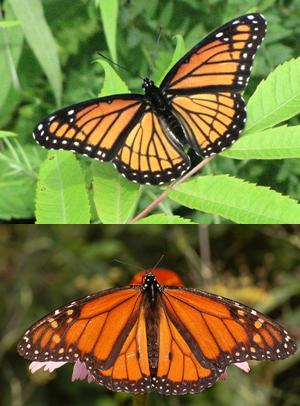
\includegraphics[scale=0.75]{images/BatesMimButter}
	\caption[A very well-known example of mimicry, the viceroy butterfly]{A very well-known example of mimicry is the viceroy butterfly (top) which has a pattern very similar to the unpalatable monarch butterfly (bottom). It was considered for a long time that this is an ideal example of Batesian mimicry. But recently Brower discovered that the viceroy is actually just as noxious as the monarch, making this a case of Mullerian mimicry. \cite{brower1991} Image source: \href{http://en.wikipedia.org/wiki/Mullerian_mimicry}{Wikipedia}}
	\label{fig:mullerian-butterfly}
\end{figure}

\section{Evolutionary Dynamics of Mimicry}
\label{sec:evolutionary-dynamics-of-mimicry}
The dynamics of mimicry has been investigated by Turner \cite{turner1988}, where he states that the evolution of mimicry can be explained best by the process of punctuated equilibrium instead of phyletic gradualism. 

\paragraph{Punctuated Equilibrium}
In evolutionary biology, punctuated equilibrium is the theory which proposes that most sexually reproducing species will remain in an extended state called \textit{stasis} while experiencing little evolutionary change for most of their geological history. When evolution occurs it is localized in rare, rapid events of branching speciation, called cladogenesis. Cladogenesis is the process by which species split into two distinct species, rather than one species gradually transforming into another. Thus, \textsl{``punctuated equilibria is a model for discontinuous tempos of change (in) the process of speciation and the deployment of species in geological time" \cite{gould1977}}. 

\paragraph{Phyletic Gradualism}
In contrast to punctuated equilibrium, phyletic gradualism states that species continue to adapt to new environmental and biological selection pressures over the course of their history, gradually becoming new species. Phyletic gradualism holds that a species population changes gradually; that is there is no clear line of demarcation between an ancestral species and a descendant species unless a splitting (cladogenetic) event occurs or the gradually-changing lineage is divided arbitrarily. During this process, evolution occurs at a smooth, steady and incremental (but not necessarily constant and slow) rate on a geological time scale. 

On this issue Turner states,

\textsl{``According to punctuated equilibrium, therefore, evolution is not more of less both gradual and continual, as has been supposed for most purposes in most post-Darwinian theories. Rather, most morphological change is held to take place within geologically short periods, separated by vastly longer periods of comparative stasis \cite{eldredge1972}. The rapid, large changes all occur during speciation, that is to say during the branching of the evolutionary tree (cladogenesis);" \cite{turner1988}}

\begin{figure}[H]
	\centering
	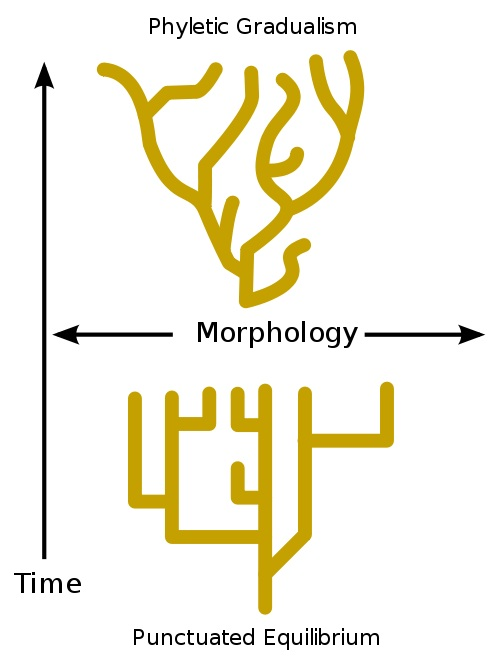
\includegraphics[scale=0.5]{images/Punctuated-equilibrium}
	\caption[Punctuated equilibrium vs. phyletic gradualism]{Punctuated equilibrium, bottom, consists of morphological stability and rare bursts of evolutionary change, while the top explains phyletic gradualism. Image source: \href{http://en.wikipedia.org/wiki/Punctuated_equilibrium}{Wikipedia}}
	\label{fig:punctuated-equilibrium}
\end{figure}

To explain the dynamic evolutionary process of mimicry, Turner came up with a synthetic theory \cite{turner1988}, which was originated by Poulton \cite{poulton1912} and Nicholson \cite{nicholson1927}, termed as the \textbf{two stage model}. This theory states that mimicry normally arises in two steps. A comparative large mutation achieves a good approximate resemblance to the model; it is followed by gradual evolutionary changes that refine the resemblance, in many cases to a high degree of perfection \cite{sheppard1972} \cite{ford1964}. This two-stage theory has been applied for the explanation of Mullerian mimicry as well.

\subsection{Mimicry Ring}
Any theory of Mullerian mimicry has to take into account the phenomenon of the coexistence of multiple mimicry rings. If we examine the local butterfly fauna in any area of the world, we will find that between all the aposomatic (warningly colored and defended) species present there are normally only a limited number of different patterns, normally far smaller than the number of species. Each cluster of species, all sharing a common pattern, is termed as Mullerian mimicry ring. Thus, in the rain forest of South and Central America, most of the long-winged butterflies (ithomiids, danaids, and heliconids) belong to one of only five different rings.

\subsubsection{Formation of Mimicry Rings}
In regards to the formation of mimicry ring Turner \cite{turner1988} has given a theory which takes into account the level of protection of different rings of butterfly species and their difference in phenotypic warning patterns. Different level of variation of these two parameter can give us very different formation of mimicry ring evolution. The cases are considered below.

\begin{itemize}
	\item If we imagine two different rings of similar warning patterns in one single habitat, similar enough that the envelop of protection afforded to one gives some protection to the more extreme variant of the other (in a simplified language, suppose that predators that have sampled species A sometimes avoid the more extreme members of species B because they mistake them as A), then these two species are subject to natural protection for mutual convergence of their patterns. Eventually they will form a rather accurate Mullerian mimicry ring.
	\item By contrast, if the two species have patterns so dissimilar that predators encountering one never imagine that it might be the other (the envelop of protection do not overlap the other species' phenotype distribution), then there is no selection whatever for convergence, and the two patterns will remain distinct indefinitely.
 \item But mutations of color patterns are occurring all the time. Suppose that species B happens to produce a mutation whole pattern falls within the envelop of protection afforded to species A. The mimicry need not be perfect, but if it is good enough, the mutation will have an advantage and will spread. In this way species B may, by a single mutation, become a Mullerian mimic of species A; in other word species B may switch from one Mullerian mimicry ring to another. Clearly, if the mimicry is not perfect, the two patterns will then gradually converge, making the resemblance ever closer. 
\end{itemize}

Like Batesian mimicry, Mullerian mimicry can evolve in two stages: the mutational, one way convergence stage followed by the gradual, mutual convergence stage. It is worth mentioning that in the first stage only the less protected species can adopt the pattern of the better protected species; mutations in the other direction is not favored.

\section{Conclusion}
Mimicry is one of the most fascinating cases of evolutionary biology. This phenomenon has been studied extensively as infinite number of evidence exists in nature. One hundred years after Bates first clearly defined the concept, a review of literature listed 1,500 papers arguing for or against it. And this figure is more than 40 years old as it has been taken from Wilcker \cite{wickler1986}, published in 1968. It is almost impossible to survey all the known examples of Mimicry, and this would in any case be pointless. Then again many examples can be found in Cott's \textit{Adaptive Coloration in Animals} \cite{cott1957}.

